\definecolor{myyellow}{rgb}{1,0.96,0.49}
\chapter{Desarrollo}
Tomando la teoría de autómatas sobre grafos computacionales como base en el desarrollo se consideran las entidades federativas del país como nodos del grafo y para formar la lista de adyacencia se considera la adyacencia geográfica, es decir, para el caso de Michoacán, se consideran los estados con los que colinda: Colima, Jalisco, Guanajuato, Estado de México y Guerrero, para hacerlo web se desarrolló en el lenguaje javascript y para mostrar un mapa interactivo de los estados se utilizó una API de google llamada Google Charts.

El grafo se forma a partir de la lista de aristas y con esta se construye la lista de adyacencia, esto para tener en todo momento la información de manera directa de los vecinos de un nodo $v$, el identificador del nodo se mapea para que cada estado tenga uno único.
\\ 
A pesar de que el modelo que se considera en \cite{cagraph} considera a cada nodo como un grupo de personas, de momento no se consideran datos reales sobre la población de cada entidad, sin embargo es algo que se puede y debe considerar para modelar correctamente la propagación de la pandemia.


\href{https://github.com/QApolo/CS/tree/master/05_CovidProj}{\textbf{Click aquí}} para ver una versión actualizada del proyecto.


\lstset{backgroundcolor=\color{myyellow}}
\lstinputlisting[language=Java,firstline = 1, lastline=51]{../src/CA.js}

\newpage

%\lstset{backgroundcolor=\color{myyellow}}

\lstset{inputencoding=utf8/latin1}
\lstinputlisting[language=Java,firstline = 1,lastline=51]{../mapExample/code.js}

\chapter{Resultados}
Como se mencionó anteriormente, no se consideraron datos reales sobre la población por entidades y específicamente fueron valores aleatorios cercanos al promedio por entidad, esto debido a la falta de tiempo para extraer los datos de una fuente confiable y que como primer paso se quería experimentar de esta manera ya que al ser un modelo SIR, este no toma  en cuenta muertes ni nacimientos lo cual aunque en conjunto parece estar lejos de un modelo real es un buen inicio y que una vez que se corrobore un comportamiento adecuado con estos datos se pueda crecer el modelo con datos reales y al agregar más variables.
\newpage

\begin{figure}[h]
	\centering
	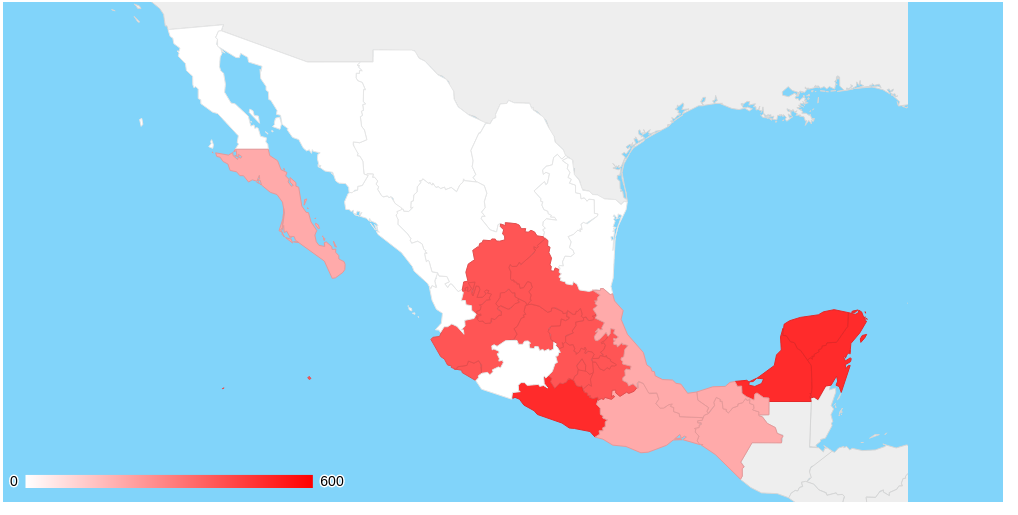
\includegraphics[width=0.5\textwidth]{capitulo2/images/map_images/Captura de pantalla_2020-06-20_15-52-04.png}
	\caption{Avance del virus extendido en el sur del país}
	\label{fig:05_prop}
\end{figure}

\begin{figure}[h]
	\centering
	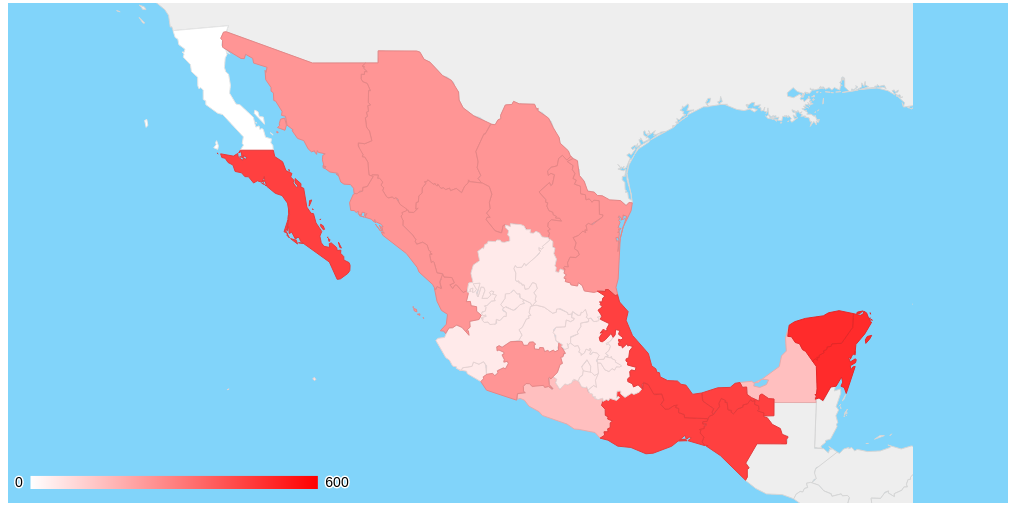
\includegraphics[width=0.5\textwidth]{capitulo2/images/map_images/Captura de pantalla_2020-06-20_15-51-33.png}
	\caption{El virus prácticamente ha alcanzado todo el territorio}
	\label{fig:02_prop}
\end{figure}
\newpage
\begin{figure}[h]
	\centering
	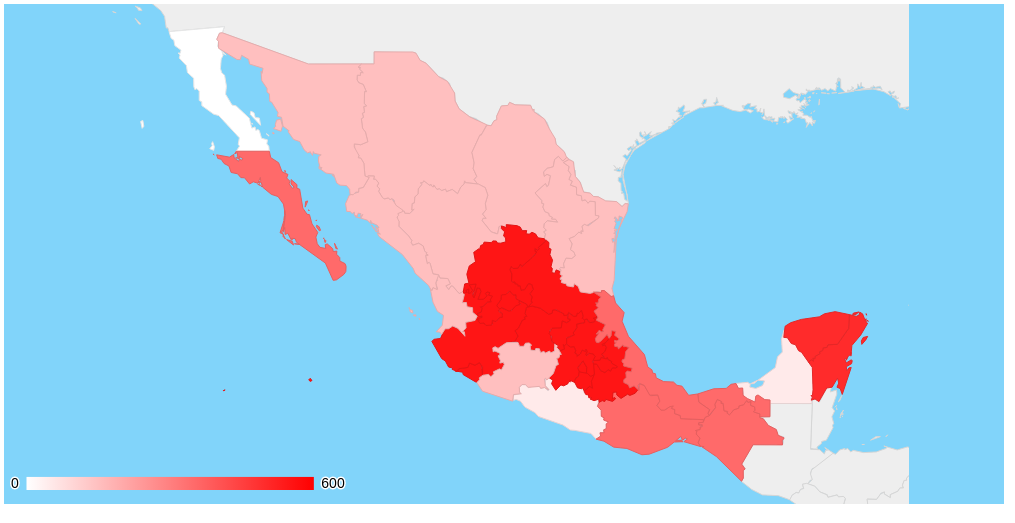
\includegraphics[width=0.5\textwidth]{capitulo2/images/map_images/Captura de pantalla_2020-06-20_15-51-23.png}
	\caption{En otro tiempo se empieza a concentrar en el bajío del país}
	\label{fig:01_prop}
\end{figure}

\begin{figure}[h]
	\centering
	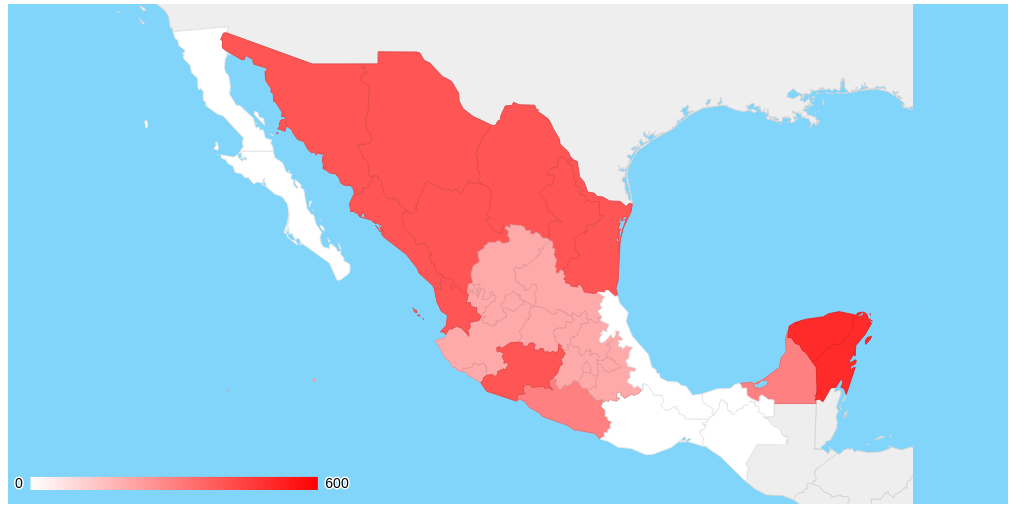
\includegraphics[width=0.5\textwidth]{capitulo2/images/map_images/Captura de pantalla_2020-06-20_15-51-45.png}
	\caption{La aparición de casos nuevos disminuye y en algunos estados no se presentan nuevos casos.}
	\label{fig:03_prop}
\end{figure}
\newpage

\begin{figure}[h]
	\centering
	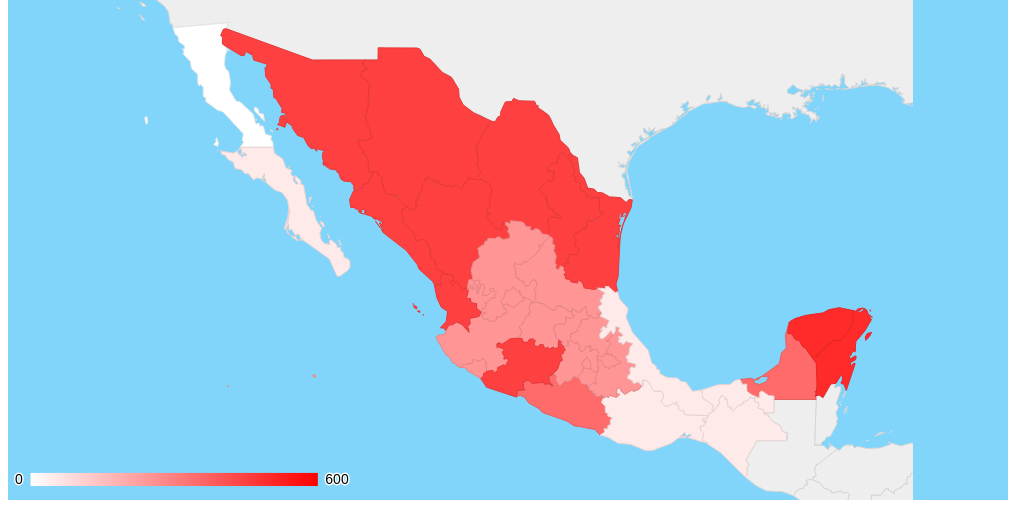
\includegraphics[width=0.5\textwidth]{capitulo2/images/map_images/Captura de pantalla_2020-06-20_15-51-52.png}
	\caption{Hay una aparente uniformidad de nuevos casos en el país.}
	\label{fig:04_prop}
\end{figure}

\begin{figure}[h]
	\centering
	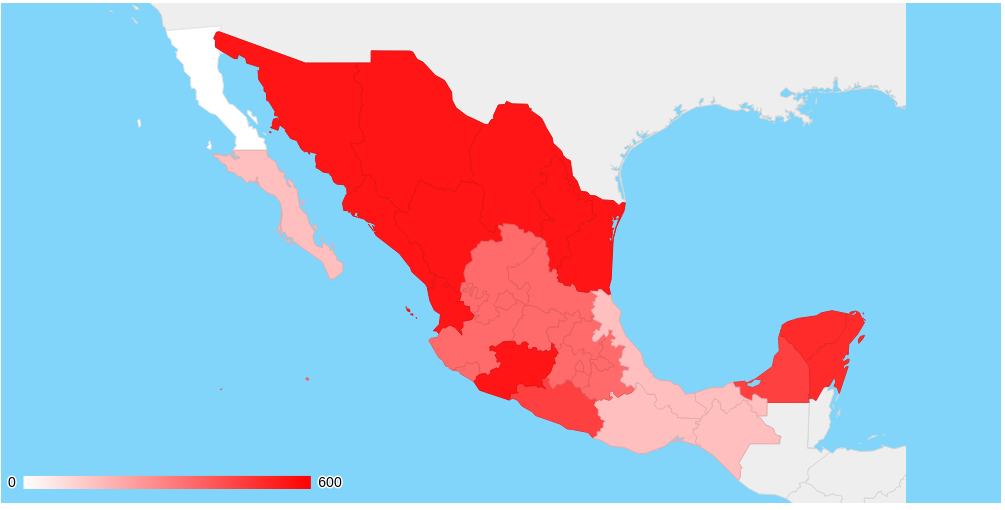
\includegraphics[width=0.5\textwidth]{capitulo2/images/map_images/Captura de pantalla_2020-06-20_15-53-01.png}
	\caption{El virus aún no se controla y tiene un patrón de crecimiento  agresivo en el norte lo que indica un rebrote.}
	\label{fig:06_prop}
\end{figure}

\href{https://qapolo.github.io/05_CovidProj/index.html}{\textbf{Ver Autómata en línea}}

Para modelar el virus de manera adecuada y tener herramientas sólidas de comparación es necesario trabajar en lo siguiente.
\begin{itemize}
	\item Cargar datos reales de la población en el país
	\item Extender el paradigma a otros modelos como SIRS o SEIR
	\item Elegir los factores que mejor se ajusten a la propagación de la pandemia real
	\item Generar gráficas en tiempo real para comparar los casos confirmados tanto acumulados como nuevos por día con las gŕáficas que presentan las autoridades.
\end{itemize}


%\section{}
% análisis
% Graficación
% Tabla rubrica

%
%\begin{figure}[h]
%	\centering
%	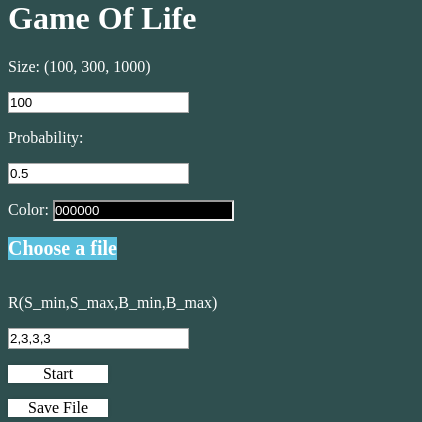
\includegraphics[width=0.7\textwidth]{capitulo2/images/menu.png}
%	\caption{Parámetros del programa}
%	\label{fig:menu}
%\end{figure}
%\newpage
